\documentclass[twoside]{article}
\usepackage{seminarpaper}
\usepackage[backend=bibtex,style=numeric]{biblatex}
\usepackage{csquotes}
\usepackage{tikz}

\usetikzlibrary{positioning}
\usetikzlibrary{matrix}

\addbibresource{references.bib}

\begin{document}

% If your paper is accepted and the title of your paper is very long,
% the style will print as headings an error message. Use the following
% command to supply a shorter title of your paper so that it can be
% used as headings.
%
%\runningtitle{I use this title instead because the last one was very long}

% If your paper is accepted and the number of authors is large, the
% style will print as headings an error message. Use the following
% command to supply a shorter version of the authors names so that
% they can be used as headings (for example, use only the surnames)
%
%\runningauthor{Surname 1, Surname 2, Surname 3, ...., Surname n}

\twocolumn[

\papertitle{Transformers in Language Models}

\paperauthor{Mikael Fredriksson}

\paperaddress{ } ]

\begin{abstract}
  The Abstract paragraph should be indented 0.25 inch (1.5 picas) on
  both left and right-hand margins. Use 10~point type, with a vertical
  spacing of 11~points.  The {\bf Abstract} heading must be centered,
  bold, and in point size 12. Two line spaces precede the
  Abstract. The Abstract must be limited to one paragraph.
\end{abstract}

\section{Introduction}
This paper will take a look at three popular language models utilizing
transformers in their architecture. It will also give a quick overview
of some applications and additions to the generic model. The aim is to
give the reader a general overview of the current landscape of different
transformer based language model architectures and some example applications.

The three different models are all similar in architecture being mostly
faithful to the original transformer architecture as presented in 
\cite{vaswani_attention_2017}. However, each of them have a different approach
to using the decoder and encoder stacks of the transformer. GPT uses only
the decoder, BERT only the encoder and T5 both encoder and decoder
\cite{radford_improving_nodate,devlin_bert_2019,raffel_exploring_2020}.

\section{Training}
All three of the models this paper discusses use transfer learning for 
training. The general idea is to first train a baseline model unsupervised 
using a large amount of unstructured text and then fine tuning the model
for each specific task after. 

The objective of the unsupervised pre-training stage is to teach the model
general language understanding. The exact details between models varies but
in general, a massive number tokens are fed into to model during the course
of training. Each word corresponds to a single or a few tokens depending on 
the encoding used [citation needed, same as pricing] and the number of tokens
used in training can go up to the trillions \cite{raffel_exploring_2020}. 
The model is asked to predict a missing token based on context. 

In the fine-tuning stage, the pre-trained model is used as a baseline. A new
model is trained using supervised learning with a task specific data set. 
The training can fine-tune all the parameters of the model, as in BERT 
\cite{devlin_bert_2019}, or an additional layer can be added and then
trained, as in GPT \cite{radford_improving_nodate}.

\subsection{Vocabulary}
Different model architectures use different vocabularies. These are chosen based
on the differing requirements of the models. The vocabulary needs to accommodate 
multiple languages and proper nouns while using as few tokens as possible per word.
Memory usage also has to be balanced and the number of tokens cannot grow infinitely
large. 

\section{Models}

The models this paper discusses very closely follow the initial architecture
presented in the paper originally proposing the transformer 
\cite{vaswani_attention_2017}. Most of the differences between 
the models come down to training.

TODO: talk about masking the attention layers somewhere, was talked about in
the t5 paper

TODO: talk about the exact differences between fine-tuning,
i think bert modifies the weights and gpt only adds an extra layer after

TODO: elmo for feature based?

\subsection{Generative Pre-Trained Transformer}
Generative Pre-Trained Transformer, more commonly known as GPT, is a model
which is focused mostly on text generation \cite{brown_language_2020}. 
GPT uses only the decoder of the transformer with 12 layers 
\cite{radford_improving_nodate}. The training is split into unsupervised
pre-training and supervised fine-tuning. 

In the unsupervised pre-training phase, the model is given a set of long form text
\cite{radford_improving_nodate}. The supervised fine-tuning is used to train the
model for a specific task. 

As the number of parameters in the model grows past a certain threshold, it
is no longer necessary to fine-tune the model for each specific use case 
\cite{brown_language_2020}. Depending on the task at hand, it might be sufficient
to just give the model some examples of the task initially and it will (understand what you want it to do). The examples are given to
the model after training during inference and thus differs from fine-tuning. 
This is called few-shot learning. Special cases of this are one-shot learning which is
otherwise similar to few-shot learning except the number of examples is one.
Zero-shot learning refers to giving the task description using natural language,
kind of like you were explaining it to a human. 

As an example \cite{brown_language_2020} used English to French translation.
The researchers gave the model between 10 to 100 pairs of examples of the
same sentence in English and French. The last pair had just an English sentence
and the model was expected to produce the corresponding sentence translated into
French.

While few-shot learning requires less data and computing power, which makes it more
accessible compared to fine-tuning a large model, at least during the writing of 
\cite{brown_language_2020} failed to produce comparable results to fine-tuning.
The number of examples given is restricted by the size of the model's context,
which for GPT-3 was 2048 tokens, around 1500 words (citation needed, pricing page has this info).

\subsection{Bidirectional Encoder Representations from Transformers}
Bidirectional Encoder Representations from Transformers, henceforth referred to as BERT,
is a language model utilizing masking of words during training to achieve bidirectionality
in the model. \cite{devlin_bert_2019}

BERT uses a similar architecture as the original transformer. It uses the encoder with
multiple layers. The main difference is in the training methods. In the pre-training step,
two different training approaches are used: masked language model and next sentence prediction.
Masking allows the self-attention layer to take into account both sides of a given word, instead
of just one side, as in GPT which can only use the previous words as context. Using next sentence
prediction improves the model's understanding of the relationships between sentences. This is
useful for question answering and natural language inference type of tasks. \cite{devlin_bert_2019}

A masked language model (MLM) is achived by hiding a certain number of tokens, 12\% in the paper, and
asking the model to predict the hidden token. The model can then use both sides of the token as
context. Some of the tokens marked for masking are instead turned 
into random tokens or kept as is. This helps prevent a difference between pre-training and fine-tuning.
Other unidirectional methods predict the entire text during training while MLM only 
does so only for the masked tokens. \cite{devlin_bert_2019}

Next sentence prediction takes a pair of sentences, \texttt{A} and \texttt{B}, and requests the model
to predict whether \texttt{B} follows \texttt{A} or not. In the paper, 50\% of the time \texttt{B} 
was the next sentence and 50\% of the time it was not. \cite{devlin_bert_2019}

BERT also uses unsupervised pre-training and supervised fine-tuning as the general training setup \cite{devlin_bert_2019}.
The largest amount of work and time is spent pre-training the model on a large set of unstructured
text. This teaches the model general language understanding. Fine-tuning can then be used to 
train the model for specific natural language tasks leveraging the existing language knowledge 
from the pre-training stage. Fine-tuning is usually a more lightweight operation than pre-training.

\subsection{Text-to-Text Transfer Transformer}
\begin{figure*}
  \centering
  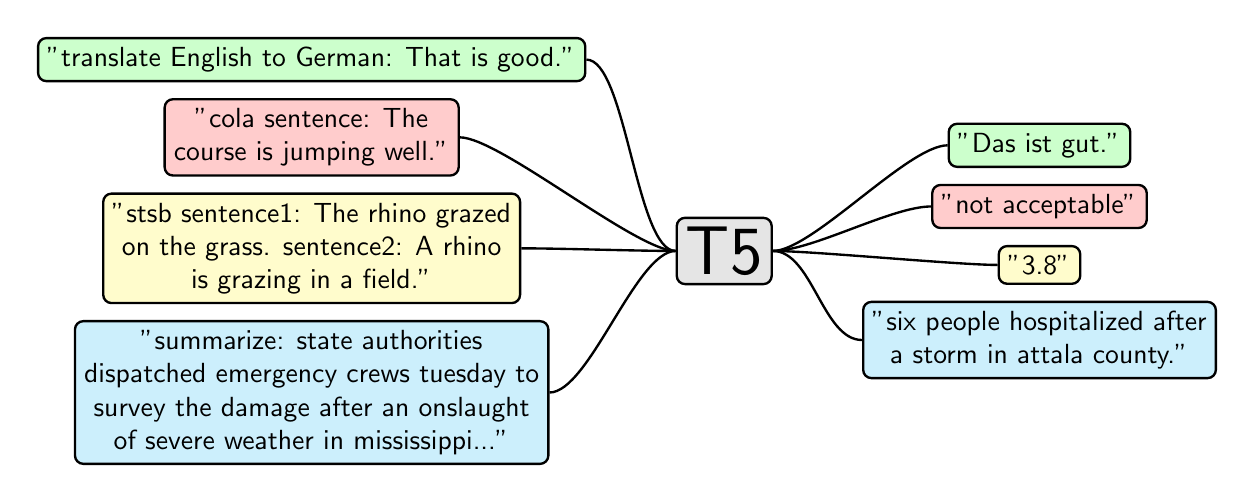
\begin{tikzpicture}[line width=0.3mm, align=center, font=\sffamily]
    % Nodes
    \matrix [matrix of nodes, row sep=2mm] (rightmat) {
      \node (translatein) [rounded corners=3pt, draw, fill=green!20] {"translate English to German: That is good."}; \\
      \node (colain)[rounded corners=3pt, draw, fill=red!20] {"cola sentence: The\\course is jumping well."}; \\
      \node (stsbin)[rounded corners=3pt, draw, fill=yellow!20] {"stsb sentence1: The rhino grazed\\on the grass. sentence2: A rhino\\is grazing in a field."}; \\
      \node (summaryin)[rounded corners=3pt, draw, fill=cyan!20] {"summarize: state authorities\\dispatched emergency crews tuesday to\\survey the damage after an onslaught\\of severe weather in mississippi..."}; \\
    };
    \node [right=of rightmat, rounded corners=3pt, draw, fill=gray!20] (t5) {\Huge T5};
    \matrix [matrix of nodes, right=of t5, row sep=2mm] {
      \node (translateout)[rounded corners=3pt, draw, fill=green!20] {"Das ist gut."}; \\
      \node (colaout)[rounded corners=3pt, draw, fill=red!20] {"not acceptable"}; \\
      \node (stsbout)[rounded corners=3pt, draw, fill=yellow!20]  {"3.8"}; \\
      \node (summaryout)[rounded corners=3pt, draw, fill=cyan!20] {"six people hospitalized after\\a storm in attala county."}; \\
    };
  
    % Lines
    \draw [-] (translatein.east) .. controls +(right:5mm) and +(left:5mm) .. (t5.west);
    \draw [-] (colain.east) .. controls +(right:5mm) and +(left:5mm) .. (t5.west);
    \draw [-] (stsbin.east) .. controls +(right:5mm) and +(left:5mm) .. (t5.west);
    \draw [-] (summaryin.east) .. controls +(right:5mm) and +(left:5mm) .. (t5.west);
  
    \draw [-] (translateout.west) .. controls +(left:5mm) and +(right:5mm) .. (t5.east);
    \draw [-] (colaout.west) .. controls +(left:5mm) and +(right:5mm) .. (t5.east);
    \draw [-] (stsbout.west) .. controls +(left:5mm) and +(right:5mm) .. (t5.east);
    \draw [-] (summaryout.west) .. controls +(left:5mm) and +(right:5mm) .. (t5.east);
  \end{tikzpicture}
  \caption{Illustrating the types of inputs and outputs. Recreated from \cite{raffel_exploring_2020}.}
\end{figure*}

Text-to-Text Transfer Transformer, abbreviated as T5, is a language model modelling each
task as text in, text out. It uses both the encoder and decoder layers of the transformer.
\cite{raffel_exploring_2020}

The main differentiating factor of T5 is the way it chooses to model tasks. Instead of 
tailoring each output to the specific task at hand, every task takes in a text prefix
describing the task and outputting the results as text. For example, for STS-B classification
task the model is trained to out one of a set of floating point numbers 
$x \in \{ 1+0.2k \mid k \in \{ 0, 1, ..., 20\} \}$ as a text. Many other models just 
output a number directly as a sliding scale from 1 to 5. 

\section{Applications}

\subsection{Toolformer}
Transformers are able to produce very natural text but as previously mentioned, they struggle with seemingly
simple tasks such as simple mathematical calculations and factual information gathering.
To get around of these limitations, transformers can be taught to use external tools
to offload these tasks to applications better suited to them. \cite{schick_toolformer_2023} 
This can be achieved using additional fine tuning, as is the case with Toolformer
\cite{schick_toolformer_2023}, or by using few-shot methods telling the model 
about the tools available to it, as in Toolformer Zero \cite{markus_toolformer_2023}.

\subsection{Multimodal Models}
Large language models have proven themselves very capable at a variety of language related
tasks. Their usefulness quickly diminishes the further we stray from their training set.
Using multimodal models (check name) however, we can widen the area of tasks the model
can complete and even achieve positive transfer, benefitting from the variety of tasks
it is trained for \cite{driess_palm-e_2023}. 

PaLM-E is a multimodal language model utilizing a transformer based language model called
PaLM \cite{chowdhery_palm_2022,driess_palm-e_2023}. Multimodality refers to the fact that
the models accept types of input other than text. For example, PaLM-E accepts an input like
"\texttt{Q: What happened between <img\_1> and <img\_2>?}" \cite{driess_palm-e_2023} where
\texttt{<img\_1>} and \texttt{<img\_2>} refer to image embeddings. The E in PaLM-E refers to
the model being embodied. This means that the model is capable of performing tasks that
relate to real world objects. For example, the model can be used to plan high-level tasks
for a robot. \cite{driess_palm-e_2023}

\begin{figure}[h]
  \centering
  \includegraphics*[scale=0.1]{img/palm-e-transfer.png}
  \caption{
    PaLM-E displays positive transfer in learning. The performance is better for these three
    distinct robotics domains when trained together than when trained separately for the 
    specific tasks. \cite{driess_palm-e_2023}
  }
\end{figure}


\section{Problems}
TODO: write about hallucination, overconfidence, radicalization etc.
For example, when asking ChatGPT, which uses a slightly modified version of GPT-3 called 
GPT-3.5 [citation needed], to do a simple calculation, it answers confidently. 
With a prompt of "\texttt{what is 491*397}" we receive a response of 
"\texttt{The product of 491 and 397 is 195127.}". Unfortunately, using a calculator
leads to a different answer: 194927. Dangerously close, but not quite there.

Another example is asking the model about something they have not been trained on, for
example about future events. Prompting the model with 
"\texttt{What did Sauli Niinistö accomplish during his third term in office?}" returns
a logically perplexing response "\texttt{Sauli Niinistö is the current President of Finland, 
and he is currently serving his second consecutive term in office. 
His third term began on March 1, 2018, and it will end on February 28, 2024. ...}".
The response claims that Sauli Niinistö is currently serving his second term in office
which is correct as of 2023 and also in 2021 where the training data of GPT-3.5 ends 
[citation needed]. However, after this, the response claims that his third term began
in 2018, directly contradicting the previous statement. It is also important to mention
that there has been a two term limit since (insert year here) written into law 
[citation needed, finlex?]. Rest of the response after the first paragraph is removed.

While these limitations can be quite clear to professionals, many people without relevant
experience have no way of discerning factually correct answers from wrong ones. The confidence
by which the models answer can also mislead people into trusting the answers too much.



\printbibliography

\end{document}
